
\chapter{An overview about vector fields}

Active contours, also called snakes, are curves that move inside the image following the energy of the field. There are two kinds of forces, one internal and anther external. Combining these two it's possible to create a curve that follows constraints gives by the forces. The  internal  and  external  forces  are  defined  so  that  the  snake  will conform to an object boundary or other desired features within an image. Snakes are widely used  in  many  applications,  including  edge  detection,  shape  modelling and segmentation. There  are  two  general  types  of  active  contour  models  in  the literature  today:  parametric active contours and geometric active contours. Typically,  the  curves  are  drawn  toward  the edges  by  potential  forces,  which  are  defined  to  be  the  negative  gradient  of  a  potential function.  Additional  forces,  such  as  pressure  forces,  together  with  the  potential  forces comprise the external forces. There are also internal forces designed to hold the curve together and to keep it from bending too  much.  There  are  two  levels  difficulties  with  active  contour  algorithms.  First,  the  initial contour must be close to the true boundary or else it will likely converge to the wrong result. The second problem is that active contours have difficulties progressing into concave  boundary  regions.  Although  many  methods  such  as  multi resolution  methods, pressure forces, distance potential forces, control points, and using solenoidal external fields have been proposed they either solve one problem or solve both but creating new difficulties. For  example,  multi resolution  methods  have  addressed  the  issue  of  initialization,  but specifying  how  the  snake  should  move  across  different  resolutions  remains  problematic. Another example is that of pressure forces, which can push an active contour into boundary concavities, but cannot be too strong or “weak” edges will be overwhelmed. But how works a snake if the objects to segment are overlapped? Snakes are able to find all the external edges of the object but in this case the edge can be consider an internal part of the object. With the active contours is impossible segment the overlapped cells because the snake cannot enter inside the cell region. For these reason we have used our virtual field following another lecture key.

\section{Vector field convolution}
Convolving a vector field with the edge of the map derived from the image you get an external force, the VFC. Active contours using the VFC external force are called VFC snakes. Like the GVF snakes instead of being Formulated using the standard energy minimization framework, VFC snakes are constructed from a state of equilibrium between the forces. The VFC snakes besides having a wide capture range and the ability to capture the concavities, are better resistant to noise image, have the ability to adapt the force field and reduce drastically the computational cost.
Before to explain the VFC is right explain the vector field kernel
\begin{equation}
 k ( x,y ) =m(x,y)n(x,y)
\end{equation}
where n is the unit vector that points to the origin of the kernel	
\begin{equation}
n ( x,y ) = [\frac{-x}{r} , \frac{-y}{r} ]
\end{equation}
and m is the magnitude of the vector . The authors of the VFC implemented two kind of magnitude. If we consider the origin as the point of interest, this vector field kernel has the desirable property that a free particle placed in the field is able to move to the point of interest. The external force that work in the VFC is defined in this way:
\begin{equation}
{f} _{vfc} ( x,y ) = {u} _{vfc} ( x,y ) , {v} _{vfc} (x,y)
\end{equation}
Since the map of the edge is non-negative and is wider near the edges of the image, the edges act to a greater extent on the VFC than homogeneous regions. Therefore, the free particles of homogeneous regions will be attracted to the edges. If we present the vector field kernel using a complex-valued range, the VFC is just the filtering result of the edge map, which does not depend on the origin of the kernel. The VFC field highly depends on the magnitude of the vector field kernel . Field VFC has the magnitude directly proportional to the vector field kernel (x, y). Knowing that the figure of interest has less influence on the particles away from it, the magnitude must be expressed as a positive function decreasing with respect to the distance of the origin. Below are propose two types of magnitude functions, given as
\begin{equation}
{m} _{1} ( x,y ) =(r+\epsilon) ^{-\gamma}
\end{equation}
\begin{equation}
{m} _{2} ( x,y ) =exp(-r^{2}\, \zeta ^{2})
\end{equation}
where $\gamma$ and $\zeta$ are positive parameters to control the decrease, $\epsilon$ is a small positive constant to prevent division by zero at the origin. ${m} _{1} ( x,y )$ is inspired by Newton’s law  of universal gravitation in physics. Furthermore, the pixels in the edge map can be considered as objects of mass proportional to the strength of the edges and the field VFC would be the gravitational field generated by all objects. The influence of the figure of interest increases as $\gamma$ decreases. In practice $\gamma$ usually ranges from 1.5 to 3 for most images. ${m} _{2} ( x,y )$ is a Gaussian shape function, where $\zeta$ can be viewed as the standard deviation. The influence of the figure of interest increases as $\zeta$ increases. In general, the influence of the figure of interest should be increased (decrease or increase) as the signal-to-noise ratio is decreased.\cite{VFC}


\section{New kind approach to segment leukocytes}
As we can see in literature, the main approach used to resolve the overlap problem is using the watershed transform. Here\ref{fig:overlap} there is an example of the watershed transform. Takes in input the image of the two overlapped circles, we calculate the distance transform, or in other words we calculate the Euclidean distance transform of the binary image BW. For each pixel in BW, the distance transform assigns a number that is the distance between that pixel and the nearest nonzero pixel of BW\ref{fig:overlaptransf}.Giving the distance transform result to the watershed algorithm we obtain a division between circles because the watershed transform finds "catchment basins" or "watershed ridge lines" in an image by treating it as a surface where light pixels represent high elevations and dark pixels represent low elevations.\ref{fig:overlapwater}
\begin{figure}[htbp]
    \centering
    \begin{subfigure}[b]{0.3\textwidth}
        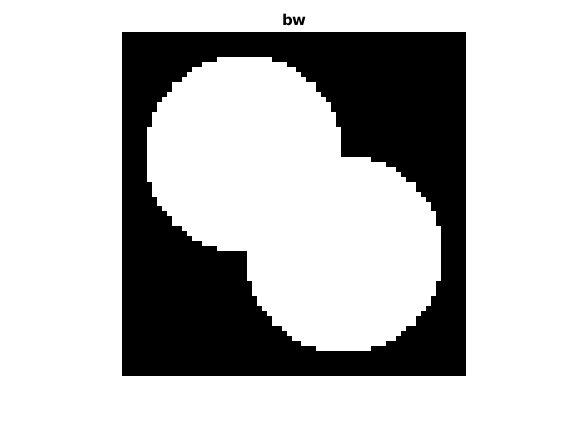
\includegraphics[width=\textwidth]{img/circlesEx.png}
        \caption{ }
        \label{fig:overlap}
    \end{subfigure}
     \quad
      %(or a blank line to force the subfigure onto a new line)
    \begin{subfigure}[b]{0.3\textwidth}
        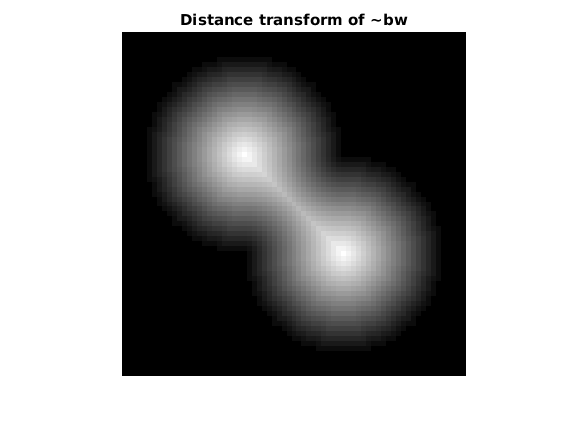
\includegraphics[width=\textwidth]{img/distancerTransform.png}
        \caption{ }
        \label{fig:overlaptransf}
    \end{subfigure}
    \quad
    \begin{subfigure}[b]{0.3\textwidth}
        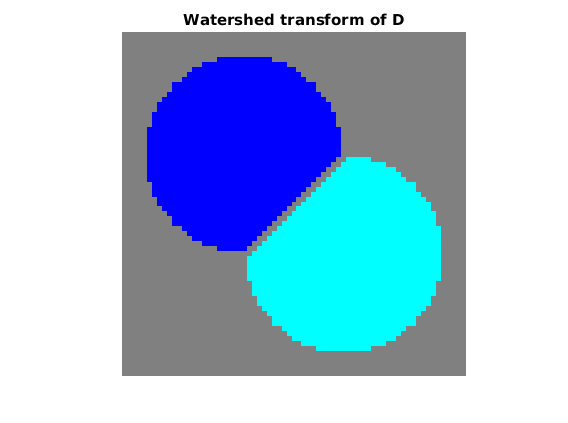
\includegraphics[width=\textwidth]{img/watershedEx.png}
        \caption{ }
        \label{fig:overlapwater}
    \end{subfigure}
    \caption{(a) Example of two circle in overlap, (b) Distance transform, (c) Watershed result}\label{fig:stepswater}
\end{figure}
This is an ideal case to analize. But when we work with the overlapping between cells the result of the division by Watershed transform is not optimal like the example \ref{fig:stepswater}. Probably the cause derived from the low definition of the figures and especially the shape of the cells. Here there is an example of what happened when we try to divide 3 cells in overlap\ref{fig:exOnImage7}.
\begin{figure}
	\centering
	\begin{subfigure}[b]{0.3\textwidth}
        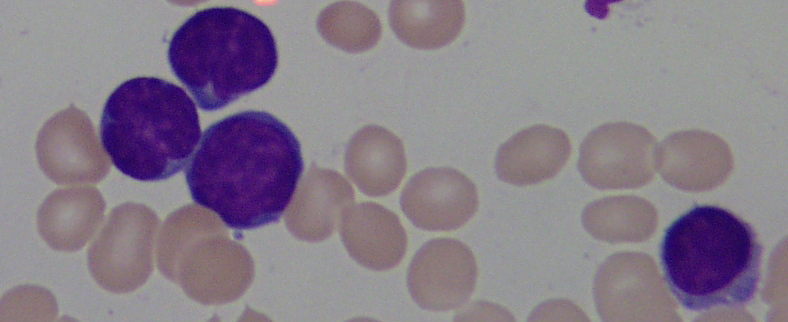
\includegraphics[width=\textwidth]{img/Im007_1_crop.png}
        \caption{ }
        \label{fig:origimage}
    \end{subfigure}
    \begin{subfigure}[b]{0.3\textwidth}
		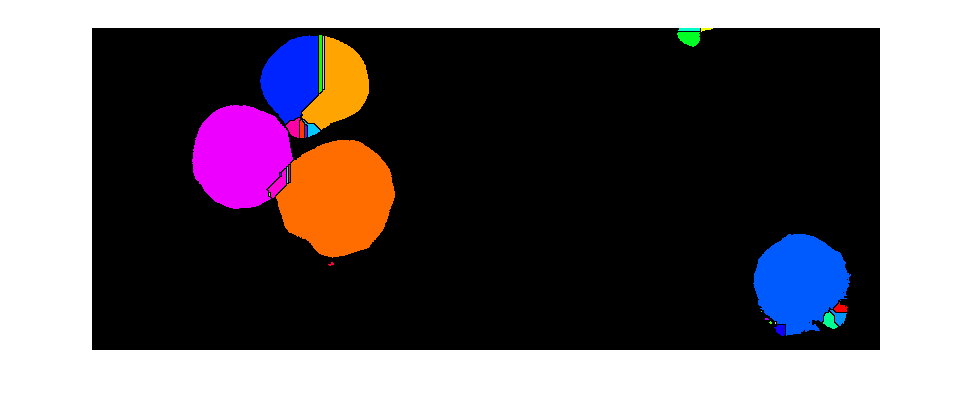
\includegraphics[width=\textwidth]{img/waterTrRes.png}
		\caption{ }
		\label{fig:watershedoncells}
	\end{subfigure}
	\caption{(a) Original leukocytes image, (b) Watershed transform applied to three cells in overlap}
	\label{fig:exOnImage7}
\end{figure}
As is possible to see, this method produce a no-realistic separation of the cells.
For this reason we study a different method that in automatic way produce a realistic division of the cells.
The algorithm uses principally the output of the VFC field, the image relative to the External energy of the image to describe the edges, the median filter and the skeleton method.
\section{The VFC result}
The VFC uses the two components of the external force ${u} _{vfc} ( x,y ) , {v} _{vfc} (x,y)$ to describe the field of the image and it's magnitude. Our purpose is find and image using these two components that describes all the leukocytes edges taking an accurate look on the edges in overlap. The first step then is extract the right component and the left component.
\begin{equation}
{u} _{vfc}=ExtF(x)/\sqrt{ExtF(x)^{2} + ExtF(y)^{2}}
\end{equation}
\begin{equation}
{u} _{vfc}=ExtF(y)/\sqrt{ExtF(x)^{2} + ExtF(y)^{2}}
\end{equation}
where ExtF is the External force of the field. Now we have only an intensity image, but to understand how the field moves in the space we have to transform these two component $ u$ and $ v $ in grades. It a mandatory do this step because we want to understand the direction of every pixel in the figure. Is possible convert the two components in degrees using the $atan2d$ function \ref{fig:angle}.
\begin{figure}
	\begin{center}
		\centering
		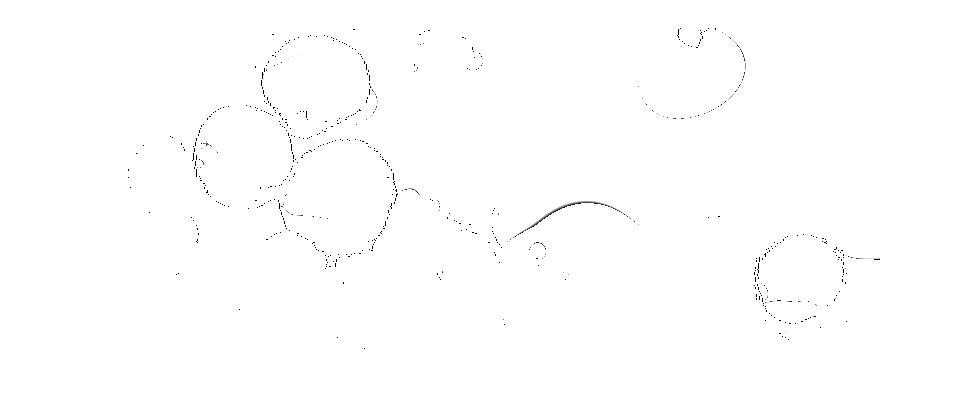
\includegraphics[scale=0.5]{img/angle.png}
		\caption{degrees image}
		\label{fig:angle}
	\end{center}
\end{figure}
In order to delete all the uniform part of the figure and put in exalt the edges we use a mediand filter using the function $ordfilt2$ searching the 18th element of the $5 * 5$ mask \ref{fig:Pmedangle}.
\begin{figure}
	\begin{center}
		\centering
		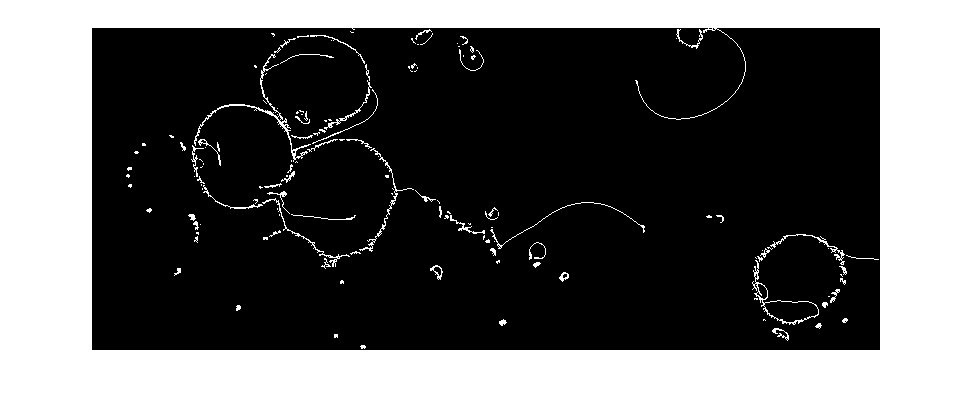
\includegraphics[scale=0.5]{img/PmedAngle.png}
		\caption{Median filter on degrees image}
		\label{fig:Pmedangle}
	\end{center}
\end{figure}
\section{External Force}
As is possible to see in the result \ref{fig:angle}, there are a lot of points that are artefacts of the field. For these reason we used the $bwdist$ function to assign a number that it is the distance between each pixel and the nearest no-zero pixel of the image. This trick is very useful because reduce the entropy of the image, focusing only on the shape of the leukocytes \ref{fig:bwdistangle}.
\begin{figure}
	\begin{center}
		\centering
		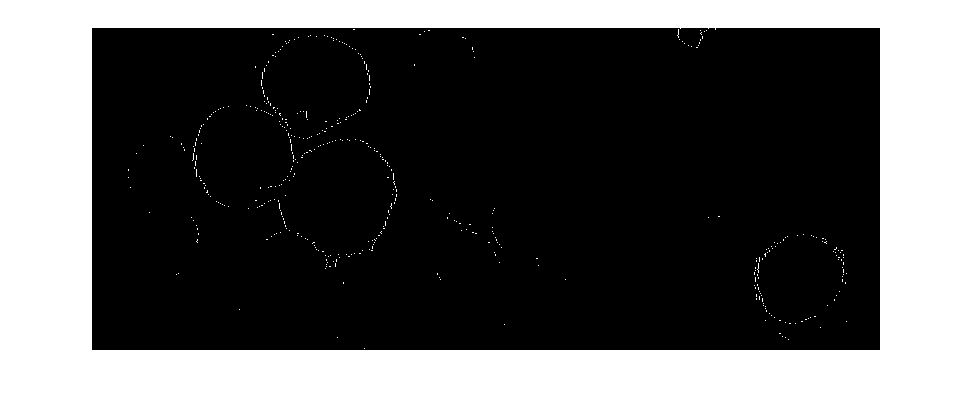
\includegraphics[scale=0.5]{img/bwdistAngle.png}
		\caption{bwdist applied on degrees image}
		\label{fig:bwdistangle}
	\end{center}
\end{figure}
